\documentclass[a4paper,10pt]{article}
%\usepackage[latin1]{inputenc} % Paquetes de idioma
\usepackage[utf8]{inputenc} % Paquetes de idioma (Este encoding toma acentos :) )
\usepackage[spanish]{babel} % Paquetes de idioma
\usepackage{graphicx} % Paquete para ingresar gráficos
\usepackage{grffile}
\usepackage{hyperref}
\usepackage{fancybox}
\usepackage{amsmath}
\usepackage{amsfonts}
\usepackage{listings}
\usepackage{float}
% Paquetes de macros de Circuitos
%\usepackage{pstricks}
\usepackage{tikz}

% Encabezado y Pié de página
\usepackage{fancyhdr} % Paquete para encabezados y pie de página
\pagestyle{fancy} % Sin esta línea no se imprimiría el encabezado en todas las páginas

\fancyhf{} %  Borra el encabezado anterior (Por defecto escribe el títutlo de la sección en la que se encuentra la hoja
\setlength{\headheight}{22.55pt}
\fancyhead[L]{
	{\textsf{Facultad de Ingenier\'ia $-$ Universidad de Buenos Aires \\ 66.44 Instrumentos Electrónicos}}
}
%\addtocounter{page}{5}
\fancyhead[R]{\thepage}

\renewcommand{\footrulewidth}{0.4pt} % Ajusta el tamaño de las líneas separadoras en el pié de página
\renewcommand{\headrulewidth}{0.4pt} % Ajusta el tamaño de las líneas separadoras en el encabezado

\fancyfoot[L]{
	{\textsf{Trabajo Pr\'actico N$^{\circ}4$}: Mediciones de impedancias} \\
	{\textsf{Integrantes: Eduardo Sanchez, Francisco Soler}}
	}
		

% Carátula del Trabajo
\title{ \author{} % Lo pongo para que el warning no moleste :p
\setlength{\unitlength}{1cm} %  Especifica la unidad de trabajo
\thispagestyle{empty}

\begin{picture}(18,0)
\put(0,0){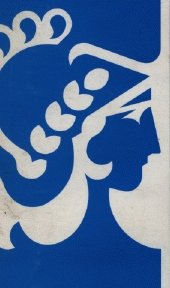
\includegraphics[width=1.5cm, height=3cm]{Logo1.png}}

\put(10.5,0){
\includegraphics[width=3cm, height=3cm]{Logo2.png}}

\end{picture}
\\[1.5cm]
\begin{center}
	\textbf{{\Huge Facultad de Ingenier\'ia \\ Universidad de Buenos Aires}}\\[2cm]
	{66.44 Instrumentos Electrónicos}\\[0.5cm]
	{Trabajo Pr\'actico N$^{\circ}3$: Mediciones de impedancias}\\[2.5cm]
\end{center}

\begin{flushleft}
	\textbf{Integrantes:} \\[1cm]

	\begin{tabular}{|c|c|c|}
		\hline
		\textbf{\normalsize Padr\'on} & \textbf{\normalsize Nombre} & \textbf{\normalsize Email} \\
		\hline
		\normalsize 92903 & \normalsize Sanchez, Eduardo Hugo & \normalsize hugo\_044@hotmail.com \\
		\hline
		\normalsize 91227 & \normalsize Soler, Jos\'e Francisco & \normalsize francisco.\_tw@hotmail.com \\
		\hline
		\normalsize xxx & \normalsize Wawrynczak, Claudio  & \normalsize claudiozak@gmail.com \\
		\hline
	\end{tabular}
\end{flushleft}
\date{} % Hace que no se imprima la fecha en la cual se compilo el .tex
 }

\begin{document}
	\maketitle % Hace que el título anterior sea el principal del documento
	\newpage

	\tableofcontents % Esta línea genera un indice a partir de las secciones y 
					 % subsecciones creadas en el documento
	\newpage


	\section{Objetivo}
	
	\indent	El objetivo del presente trabajo práctico es familiarizarse con 
	el qmetro, el RLC meter, el impedancímetro vectorial. Dicho instrumental
	sirve para medir impedancias. Luego de realizas las experiencias se 
	intentará determinar en qué circunstancias conviene utilizar uno en vez 
	de otro.

	\newpage
	\section{Desarrollo}
	
	\indent Para llevar a cabo las mediciones, se utilizan los siguientes 
	instrumentos:
		\begin{itemize}
			\item algo
			\item algo
			\item algo
			\item Cable coaxil para realizar las distintas conexiones entre 
			instrumentos.
		\end{itemize}	
	
		\subsection{Mediciones con el Q-metro}
		\subsubsection{Inductancia de una bobina con n\'ucleo de aire}
		
		\indent El circuito simplificado de un Q-metro se muestra en la Figura
		\ref{img001}

			\begin{figure}[!htb]
				\centering
				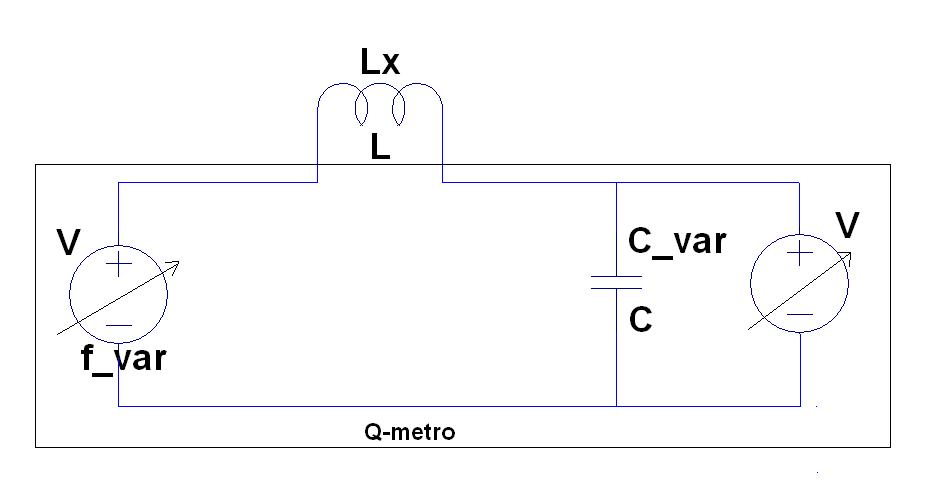
\includegraphics[width=8cm]
				{Imagenes/qmetro.png}
				\caption{Esquema simplificado del Q-metro}
				\label{img001} 
			\end{figure}

		\indent Como es un circuito serie, la máxima corriente se obtiene en 
		la resonancia, dado que la reactancia inductiva de la bobina se 
		cancela con la capacitiva. Si fuesen componentes ideales, la corriente
		sería infinita y los valores de tensiones de la bobina y del capacitor
		serían $+\infty$ y $-\infty$ respectivamente. \\
		\indent Como no son componentes ideales, los mismos tienen pérdidas y
		se las modelizan con una resistencia, por ende, la corriente no es 
		infinita. La respectiva tensión del capacitor en situación de 
		resonancia es $V_c = \frac{X_L\cdot V}{R}$. \\
		\indent Como el valor de Q es $Q=\frac{\omega L}{R}$, se observa que 
		$$V_c = Q \cdot V$$

		\indent La frecuencia de resonancia se la puede determinar de la 
		siguiente forma
		$$|X_L|=|X_C| \Rightarrow w\cdot L = \frac{1}{w\cdot C}$$

		$$f=\frac{1}{2\pi\sqrt{LC}}$$ 
		
		\indent Conocidos los valores de la capacidad, $C$, y la frecuencia, 
		$f$, puede obtenerse el valor de la inductancia de $L_x$ y tambi\'en 
		su resistencia serie equivalente con las siguientes expresiones
		$$L=\frac{1}{(2\pi)^2 f^2C}$$
		$$R_s=\frac{2\pi\cdot f\cdot L}{Q}$$
		\indent En la tabla \ref{tab001} se muestran los resultados obtenidos
		para un inductor realizando un barrido de frecuencias
		
		%Faltan incertezas jeje -----> hacete el vivo ¬¬
		\begin{table}[!htp]
					\centering
					\begin{tabular}{|c|c|c|c|c|}
						\hline
			    		Frecuencia & C & Q & L (calculado) & $R_s$ (calculado) \\
						\hline
						$13.3~MHz$& $25~pF$& 182 & $5.73~\mu Hy$ &$ 2.63~\Omega$ \\
						\hline
						$10.7~MHz$& $40~pF$& 200 & $5.54~\mu Hy$ &$ 1.86~\Omega$ \\
						\hline
						$9.6~MHz$& $50~pF$& 200 & $5.50~\mu Hy$ &$ 1.66~\Omega$ \\
						\hline  
						$6.9~MHz$& $100~pF$& 195 & $5.33~\mu Hy$ &$ 1.18~\Omega$ \\
						\hline  										
						$4.0~MHz$& $305~pF$& 170 & $5.20~\mu Hy$ &$ 0.77~\Omega$ \\
						\hline
						$3.2~MHz$& $470~pF$& 155 & $5.17~\mu Hy$ &$ 0.68~\Omega$ \\
						\hline  						  	  
					\end{tabular}
					\caption{Mediciones con el Q-metro} \label{tab001}
				\end{table}
		\subsection{Mediciones con el RLC}		
		
		\subsubsection{Inductancia de una bobina con n\'ucleo de aire}
		En la Tabla \ref{tabRLCbobina} se puede observar los resultados obtenidos de la medici\'on de una bobina con nucleo de aire a diferentes frecuencias.
		\begin{table}[!htp]
					\centering
					\begin{tabular}{|c|c|c|c|}
						\hline
			    		Frecuencia & Q & L  & R (calculado) \\
						\hline
						$100~kHz$& 36.58 & $5.23~\mu Hy$ &$ 25.5~m\Omega$ \\
						\hline
						$66.66~kHz$& 29.44 & $5.26~\mu Hy$ &$ 31.8~m\Omega$ \\
						\hline
						$50~kHz$& 25.11 & $5.29~\mu Hy$ &$ 42.1~m\Omega$ \\
						\hline  
						$40~kHz$& 22.42 & $5.31~\mu Hy$ &$ 50.4~m\Omega$ \\
						\hline  										
						$28.572~kHz$& 19.07 & $5.35~\mu Hy$ &$ 59.5~m\Omega$ \\
						\hline
						$20~kHz$& 16.1 & $5.40~\mu Hy$ &$ 66.2~m\Omega$ \\
						\hline  
						$10~kHz$& 10.78 & $5.46~\mu Hy$ &$ 74.8~m\Omega$ \\
						\hline 										
						$1~kHz$& 1.36 & $5.53~\mu Hy$ &$ 89.8~m\Omega$ \\
						\hline 	  
					\end{tabular}
					\caption{Mediciones con el RLC} \label{tabRLCbobina}
				\end{table}
						
		\subsubsection{Capacidad de un capacitor electro\'itico}	
		\subsubsection{Capacidad de un capacitor cer\'amico}
		
		\subsection{Mediciones con el puente de impedancias}
		En la Tabla \ref{tabPUENTEbobina}
		\begin{table}[!htp]
					\centering
					\begin{tabular}{|c|c|c|c|c|}
						\hline
			    		Frecuencia & Q & L  & R (calculado) \\
						\hline
						$20~kHz$& 20 & $5.10~\mu Hy$ &$ 32~m\Omega$ \\
						\hline
						$1~kHz$& 1.8 & $6.30~\mu Hy$ &$ 22~m\Omega$ \\
						\hline	  
					\end{tabular}
					\caption{Mediciones con el RLC} \label{tabPUENTEbobina}
				\end{table}	
		\subsubsection{Inductancia de una bobina con n\'ucleo de aire}
		
		\subsection{Mediciones con el impedanc\'imetro}
		\subsubsection{Frecuencia de resonancia de una bobina con n\'ucleo de aire}
		\subsubsection{Inductancia de una bobina con nucleo de ferrite}
		En la Tabla \ref{tabIMPbobina}
		\begin{table}[!htp]
					\centering
					\begin{tabular}{|c|c|c|c}
						\hline
			    		Frecuencia & |Z| & arg(Z)  & L (calculado) \\
						\hline
						$25.5~MHz$ & $160~\Omega$ & $90^{\circ}$ & $0.99~\mu Hy$ \\
						\hline
						$42~MHz$ & $260~\Omega$ & $90^{\circ}$ & $0.98~\mu Hy$\\
						\hline
						$44.8~Hz$ & $300~\Omega$ & $85^{\circ}$ & $1.06~\mu Hy$ \\
						\hline
						$58.2~Hz$ & $430~\Omega$ & $78^{\circ}$ & $1.17~\mu Hy$ \\
						\hline									
						$69.5~Hz$ & $560~\Omega$ & $72^{\circ}$ & $1.28~\mu Hy$ \\
						\hline									
						$80.0~Hz$& $640~\Omega$ & $55^{\circ}$ & $1.27~\mu Hy$ \\
						\hline									
						$84.0~Hz$ & $550~\Omega$ & $45^{\circ}$ & $1.04~\mu Hy$ \\
						\hline									
						$93.0~Hz$ & $430~\Omega$ & $70^{\circ}$ & $0.73~\mu Hy$ \\
						\hline									
						$100.0~Hz$ & $750~\Omega$ & $65^{\circ}$ & $1.19~\mu Hy$ \\
						\hline			
					\end{tabular}
					\caption{Mediciones con el RLC} \label{tabIMPbobina}
				\end{table}	
					
		\subsubsection{Param\'etros de una l\'inea de transmisici\'on}
		Como la impedancia de entrada de una l\'inea de transmisi\'on (la que mide el impedanc\'imetro) est\'a dada por $$Z_{in}=Z_0\frac{Z_L+Z_0\tanh(\gamma L)}{Z_0+Z_L\tanh(\gamma L)}$$
		Suponiendo que la l\'inea es de bajas p\'erdidas $\gamma=\alpha+j\beta=j\beta=j\frac{2\pi}{\lambda}$ y si adem\'as se impone la condici\'on de que $L=\frac{\lambda}{8}$ entonces la expresi\'on de la impedancia de entrada se reduce a la siguiente
		$$Z_{in}=Z_0\frac{Z_L+jZ_0}{Z_0+jZ_L}$$
		Si $Z_L= 0$ entonces $Z_{in}=jZ_0$ \\
		Si $Z_L \rightarrow \infty$ entonces $Z_{in}\rightarrow-jZ_0$
		Entonces conectando una l\'inea al impedanc\'imetro a una frecuencia adecuada y dejando el extremo libre de la l\'inea cortocircuitado o abierto se obtiene el valor de la impedancia de la l\'inea, la cual es de $Z_0=75~\Omega$ ($f=7.9~MHz$ $L=3~m$)
		
		Por otra parte se si se elije $L=\frac{\lambda}{2},3\frac{\lambda}{2}, 5\frac{\lambda}{2} ...$ y que $Z_L\rightarrow\infty$, entonces puede obtenerse la atenuaci\'on de la l\'inea
		$$Z_{in}=Z_0\frac{Z_L+Z_0\alpha L}{Z_0+Z_L\alpha L}=\frac{Z_0}{\alpha L}$$
		Despejando la atenuaci\'on de la l\'inea se obtiene
		$$\alpha=\frac{Z_0}{Z_{in} L}$$
		o la atenuaci\'on en decibles cada $100~m$
		$$\alpha=\frac{Z_0\cdot8.69~dB}{100Z_{in} L}$$
		
		Con la misma l\'inea de  $3~m$ con una frecuencia de $32~MHz$ se obtuvo una $Z_{in}=2750~\Omega$ con lo cual $\alpha=80 mdB/m$
		\subsubsection{Par\'ametros de un cristal}	
		\subsubsection{Mediciones en un circuito activo}
			
	\section{Conclusiones}
	\indent Viva Venezuela!\\
\end{document}

